%% ============================================================================
%% Paper 3: Supplementary Material
%% Target: Journal of Cheminformatics
%%% ============================================================================

\documentclass[11pt,a4paper]{article}

% Page layout
\usepackage[a4paper,margin=2.5cm]{geometry}

% Fonts and encoding
\usepackage[T1]{fontenc}
\usepackage[utf8]{inputenc}
\usepackage{lmodern}

% Mathematics
\usepackage{amsmath, amsfonts, amssymb, mathtools}

% Figures and tables
\usepackage{graphicx}
\usepackage{booktabs, tabularx, array, longtable}
\usepackage{algorithm, algorithmic}
\usepackage[table]{xcolor}

% Units and SI
\usepackage[
  detect-all           = true,
  group-minimum-digits = 4,
  per-mode             = symbol,
  range-phrase         = {--},
  range-units          = single,
]{siunitx}
\DeclareSIUnit\angstrom{\text{\AA}}
\DeclareSIUnit\molar{M}
\DeclareSIUnit\kcalmol{kcal\,mol^{-1}}
\DeclareSIUnit\percent{\%}

% Hyperlinks
\usepackage[authoryear,round]{natbib}
\usepackage{xr-hyper}
\usepackage[hypertexnames=false,colorlinks=true,linkcolor=blue,citecolor=blue,urlcolor=blue]{hyperref}

% Cross-referencing
\usepackage{cleveref}
\crefname{table}{Table}{Tables}
\Crefname{table}{Table}{Tables}
\crefname{figure}{Figure}{Figures}
\Crefname{figure}{Figure}{Figures}

% Cross-reference to main manuscript
\externaldocument[M-]{Paper3_Quantum_InspiredV2608}

% Supplementary figure numbering (Figure S1, S2, ...)
\renewcommand{\thefigure}{S\arabic{figure}}
\renewcommand{\thetable}{S\arabic{table}}

% Author information
\usepackage{authblk}

% Caption styling
\usepackage[labelfont=bf,textfont={footnotesize,it}]{caption}

% Path configuration
\graphicspath{{Graphics/}}

% AUTHOR INFORMATION

\title{\textbf{Supplementary Material}\\Do topological and quantum-inspired molecular representations add value?}

\author[1]{Myke Vital Sao Temgoua}
\author[1]{Jean-Pierre Tchapet Njafa}
\author[1]{Serge Guy Nana Engo}
\author[2]{Penabei Samafou}
\author[3]{Wilfred Fon Mbacham}

\affil[1]{Department of Physics, Faculty of Science, University of Yaound\'e I, P.O. Box 812, Yaound\'e, Cameroon}
\affil[2]{Department of Medical Imaging and Radiation Sciences, Universit\'e de Sherbrooke, Sherbrooke, QC, Canada}
\affil[3]{Department of Biochemistry, Faculty of Science, University of Yaound\'e I, P.O. Box 812, Yaound\'e, Cameroon}

\date{\today}

% BEGIN DOCUMENT

\begin{document}

\maketitle

% H$_1$ PERSISTENCE AND RESISTANCE RESILIENCE SCORE

\section{Topological persistence and resistance resilience}

This supplementary analysis tests whether the topological features introduced in the main manuscript carry an association with computational resistance-resilience scores (RRS) beyond molecular size and related structural covariates. It includes $n=\num{494}$ compounds with complete H$_1$ and RRS profiles; the analysis is exploratory and is not used to claim an independent topological biomarker.

\begin{figure}[htbp]
\centering

\includegraphics[width=0.85\textwidth]{h1_rrs_class_violin.png}
\caption{H$_1$--RRS analysis. The violin plot shows the exploratory subset; class-level differences are not interpreted as independent effects. In the expanded cohort ($n = \num{494}$), H$_1$ count showed a weak unadjusted association with continuous RRS (Spearman $\rho = \num{0.2399}$, $p = \num{6.76e-8}$), but the partial association was null after controlling for molecular weight, ring count, fraction sp$^3$, and H$_0$ count ($\rho_{\text{partial}} = \num{0.0329}$, $p = \num{0.4668}$). The result is size-mediated and hypothesis-generating, not evidence of an independent topological predictor.}
\label{fig:h1_rrs}
\end{figure}




\section{Pharmacophore fingerprint representation}
\label{sec:phco_representation}

The two-dimensional pharmacophore (PHCO) baseline uses RDKit's \texttt{SparseBitVect} representation. Active bit positions were transferred explicitly to the numerical feature matrix before cross-validation. Under this representation, PHCO achieved an AUC of \num{0.896} on the \num{19836}-molecule complete-embedding panel (\cref{M-tab:benchmark}).

\section{Per-fold activity-prediction estimates}
\label{sec:per_fold}

 \cref{tab:sm_s4_perfold} gives per-fold AUC, accuracy, and F1 for six representation methods. ECFP4, TFP, and TNE use the \num{19836}-molecule complete-embedding panel; the hybrid uses the corresponding full analysis panel; QKS and RBF use a \num{5000}-molecule 6-qubit quantum-kernel panel. Summary estimates are given in the main manuscript (\cref{M-tab:benchmark}).

\begin{table}[htbp]
\centering
\caption{Per-fold activity-prediction statistics for six representation methods. ECFP4, TFP, and TNE use the \num{19836}-molecule Random Forest benchmark; the hybrid uses the corresponding Random Forest analysis; QKS and RBF use the \num{5000}-molecule 6-qubit state-vector SVM analysis. Because the rows differ in population and classifier, they are presented as complementary summaries rather than as a direct cross-method comparison. Summary estimates from the primary benchmark are given in the main manuscript (\cref{M-tab:benchmark}).}
\label{tab:sm_s4_perfold}
\small
\begin{tabularx}{\textwidth}{l l S[table-format=1.3] S[table-format=1.3] S[table-format=1.3]}
\toprule
Method & Fold & {AUC} & {Accuracy} & {F1} \\
\midrule
ECFP4 & 1 & 0.947 & 0.898 & 0.933 \\
ECFP4 & 2 & 0.950 & 0.894 & 0.930 \\
ECFP4 & 3 & 0.948 & 0.895 & 0.930 \\
ECFP4 & 4 & 0.952 & 0.899 & 0.934 \\
ECFP4 & 5 & 0.940 & 0.893 & 0.930 \\
\midrule
Hybrid (TFP+TNE+QK) & 1 & 0.894 & 0.848 & 0.902 \\
Hybrid (TFP+TNE+QK) & 2 & 0.887 & 0.844 & 0.900 \\
Hybrid (TFP+TNE+QK) & 3 & 0.886 & 0.844 & 0.900 \\
Hybrid (TFP+TNE+QK) & 4 & 0.893 & 0.846 & 0.902 \\
Hybrid (TFP+TNE+QK) & 5 & 0.878 & 0.836 & 0.895 \\
\midrule
TFP (TDA) & 1 & 0.881 & 0.846 & 0.902 \\
TFP (TDA) & 2 & 0.875 & 0.836 & 0.895 \\
TFP (TDA) & 3 & 0.880 & 0.846 & 0.902 \\
TFP (TDA) & 4 & 0.878 & 0.838 & 0.897 \\
TFP (TDA) & 5 & 0.866 & 0.826 & 0.889 \\
\midrule
TNE ($d=8$) & 1 & 0.720 & 0.753 & 0.856 \\
TNE ($d=8$) & 2 & 0.722 & 0.756 & 0.857 \\
TNE ($d=8$) & 3 & 0.733 & 0.755 & 0.857 \\
TNE ($d=8$) & 4 & 0.721 & 0.758 & 0.858 \\
TNE ($d=8$) & 5 & 0.714 & 0.760 & 0.859 \\
\midrule
QKS (quantum, 6q) & 1 & 0.791 & 0.813 & 0.881 \\
QKS (quantum, 6q) & 2 & 0.843 & 0.815 & 0.881 \\
QKS (quantum, 6q) & 3 & 0.833 & 0.826 & 0.890 \\
QKS (quantum, 6q) & 4 & 0.800 & 0.818 & 0.887 \\
QKS (quantum, 6q) & 5 & 0.833 & 0.841 & 0.900 \\
\midrule
RBF (gamma-tuned) & 1 & 0.812 & 0.821 & 0.886 \\
RBF (gamma-tuned) & 2 & 0.839 & 0.815 & 0.881 \\
RBF (gamma-tuned) & 3 & 0.844 & 0.833 & 0.894 \\
RBF (gamma-tuned) & 4 & 0.818 & 0.827 & 0.892 \\
RBF (gamma-tuned) & 5 & 0.818 & 0.843 & 0.900 \\
\bottomrule
\end{tabularx}
\end{table}

Complete per-fold records are included in the supplementary data archive.

\section{Interpretation and cross-study scope}
\label{sec:interpretation_scope}

The TNE docking analysis measures information retention on the molecular set used to derive the embeddings; it does not assess prospective binding to new compounds. TNE was competitive with ECFP4 for PfDHFR (TNE $R^2 = \num{0.473}$ versus ECFP4 $R^2 = \num{0.461}$) but lower for PfATP4 and PfCRT; these target-specific results are therefore descriptive and do not establish a universal advantage. The expanded H$_1$--RRS analysis is hypothesis-generating: the unadjusted association is attenuated after adjustment for molecular size and related structural covariates, so no independent topological predictor is claimed. The four-complex P2 MD cohort is distinct from the P3 representation panel, and the present analysis does not provide experimental activity measurements; target-level computational scores should not be conflated with systems-level mechanism-of-action evidence \citep{Trapotsi2022MoA}.

\section{Topological fingerprint statistics}



Detailed topological fingerprint statistics for the full library are provided in \cref{SM-tab:tda_stats}, and representative persistence diagrams are shown in \cref{SM-fig:persistence}.



\begin{table}[htbp]
\centering
\caption{Topological fingerprint statistics across \num{19849} valid molecules (Vietoris--Rips persistent homology, three homology dimensions).}
\label{SM-tab:tda_stats}
\begin{tabularx}{\textwidth}{l S[table-format=1.4] S[table-format=1.4] S[table-format=1.4] S[table-format=1.4]}
\toprule
Feature & {Mean} & {Std} & {Min} & {Max} \\
\midrule
H$_0$ entropy & 3.5781 & 0.2014 & 2.2887 & 4.1943 \\
H$_0$ count & 38.0417 & 7.3468 & 11.0000 & 69.0000 \\
H$_0$ max persistence (\si{\angstrom}) & 2.7166 & 0.6726 & 1.4800 & 5.9491 \\
H$_0$ mean persistence (\si{\angstrom}) & 1.6137 & 0.0644 & 1.0986 & 2.0281 \\
\midrule
H$_1$ entropy & 1.6354 & 0.3352 & -0.0000 & 2.7234 \\
H$_1$ count & 3.6058 & 1.3429 & 1.0000 & 10.0000 \\
H$_1$ max persistence (\si{\angstrom}) & 1.3916 & 0.0583 & 0.6238 & 2.7075 \\
H$_1$ mean persistence (\si{\angstrom}) & 0.6138 & 0.1341 & 0.2356 & 1.4000 \\
\midrule
H$_2$ entropy & 0.6955 & 0.3527 & -0.0000 & 1.9579 \\
H$_2$ count & 0.0304 & 0.1771 & 0.0000 & 4.0000 \\
H$_2$ max persistence (\si{\angstrom}) & 0.4672 & 0.0505 & 0.0000 & 1.2400 \\
H$_2$ mean persistence (\si{\angstrom}) & 0.3844 & 0.0892 & 0.0000 & 1.0533 \\
\bottomrule
\end{tabularx}
\end{table}



\begin{figure}[htbp]
\centering
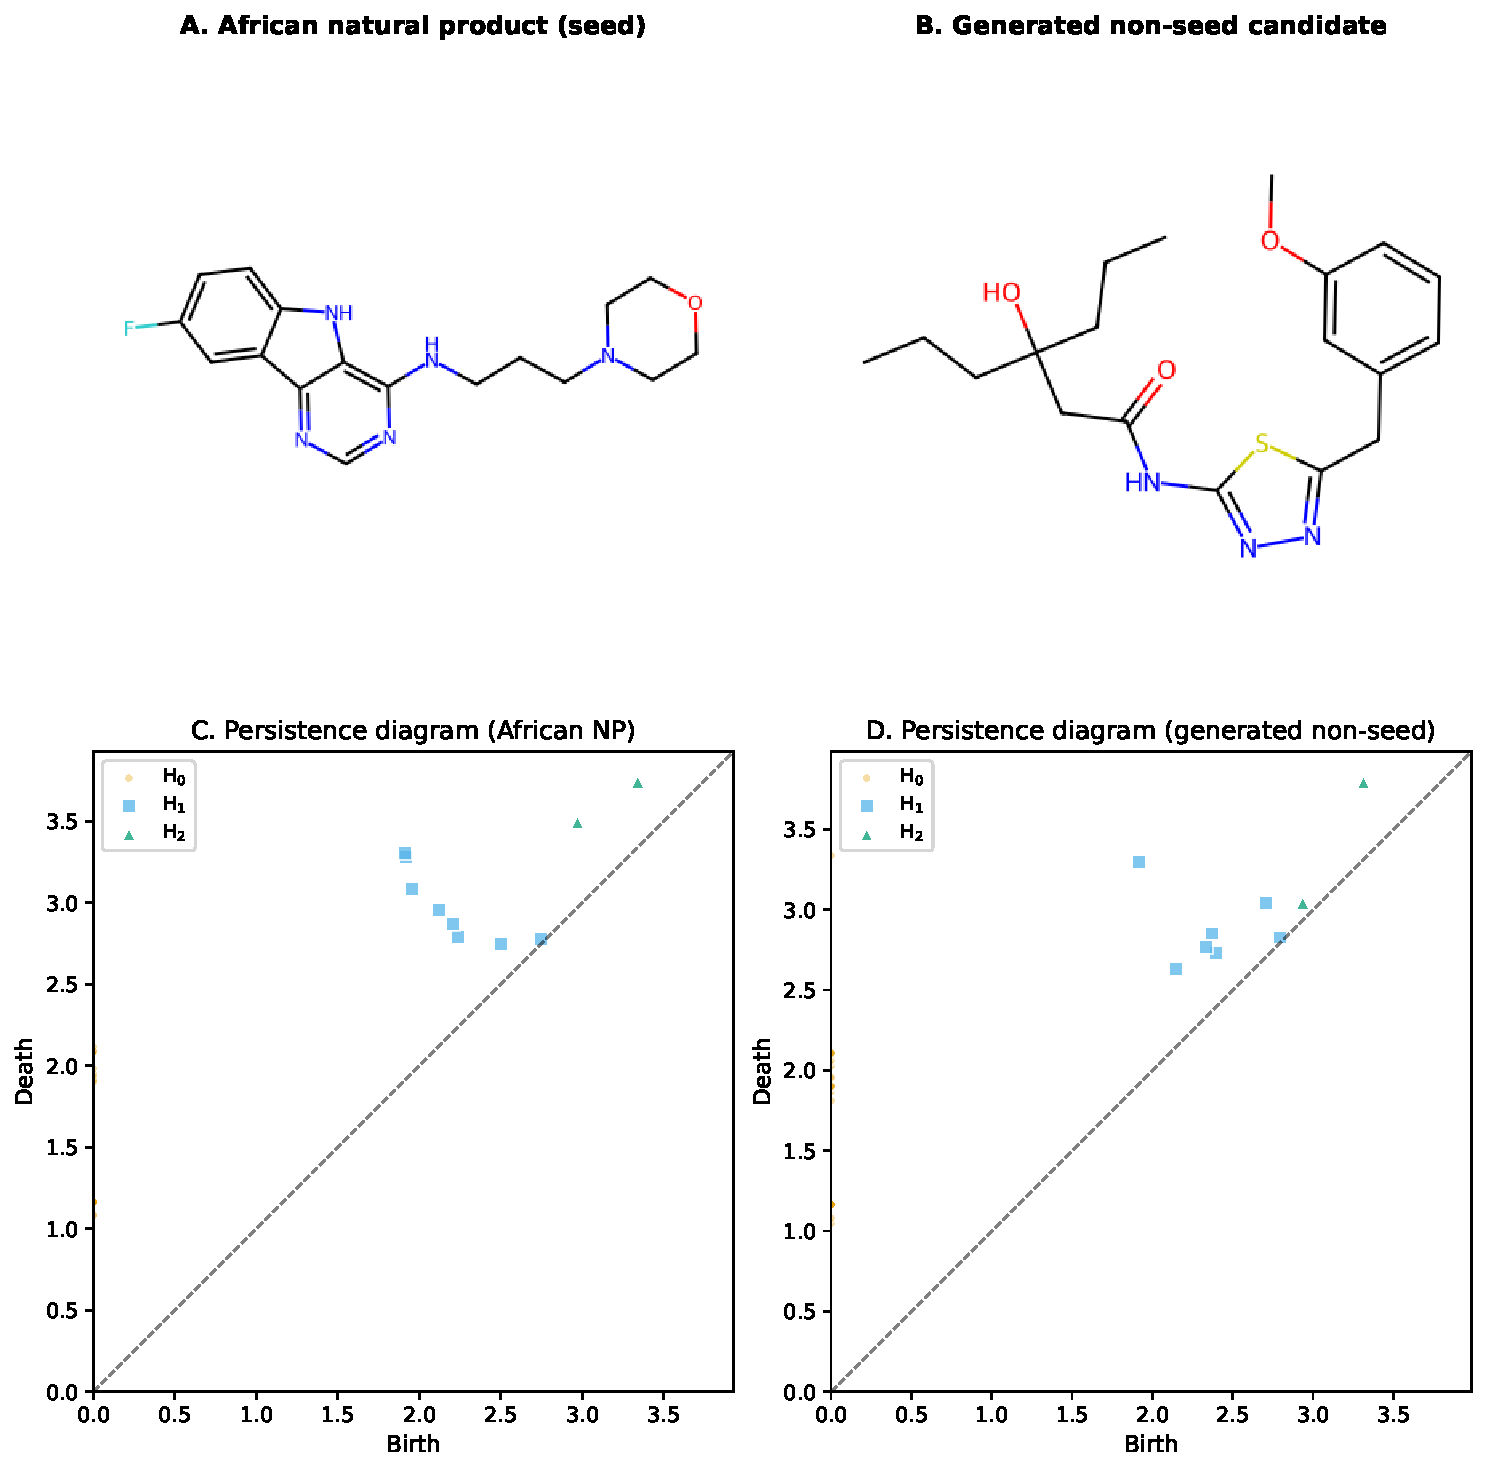
\includegraphics[width=0.75\textwidth]{persistence_diagrams.pdf}
\caption{Representative topological fingerprints of an African natural product seed and a generated non-seed candidate. (A~--~B)~2D structures of the representative molecules. (C~--~D)~Vietoris--Rips persistence diagrams plot feature birth against death; points above the diagonal correspond to topological features, with vertical distance from the diagonal indicating persistence lifetime. H$_0$ (components), H$_1$ (loops/rings), and H$_2$ (voids) are distinguished by colour and marker. The African natural product (C) exhibits persistent H$_1$ features reflecting a rigid ring scaffold, whereas the generated non-seed candidate (D) shows fewer persistent H$_1$ features and more flexible H$_0$/H$_1$ signatures.}
\label{SM-fig:persistence}
\end{figure}






\section{Clustering quality metrics}



\cref{SM-tab:clustering} reports clustering quality metrics for the three representations.



\begin{table}[htbp]
\centering
\caption{Clustering quality metrics for TNE embeddings versus VAE latent space and ECFP4 fingerprints (KMeans, $k = 484$). Higher Silhouette coefficient indicates better cluster coherence.}
\label{SM-tab:clustering}
\begin{tabularx}{\textwidth}{l S[table-format=1.3]}
\toprule
Descriptor & {Silhouette} \\
\midrule
TNE ($d=8$, \num{192}-dim) & 0.350 \\
VAE latent (\num{64}-dim) & 0.229 \\
ECFP4 (\num{2048}-dim) & 0.180 \\
\bottomrule
\end{tabularx}
\end{table}





\section{Discriminator benchmark for structural expansion}

We compared classical fingerprint similarity with quantum-kernel density in \cref{SM-tab:ga_discriminator} and \cref{SM-fig:ga_discriminator}.

\begin{table}[htbp]
\centering
\caption{Chemical similarity versus quantum kernel density benchmark: AUC-ROC comparison between ECFP4 Tanimoto distance and quantum kernel density for distinguishing $N$ expanded molecules from \num{200} reference seeds.}
\label{SM-tab:ga_discriminator}
\begin{tabularx}{\textwidth}{l S[table-format=1.4] S[table-format=1.4] S[table-format=-1.4]}
\toprule
{$N$ expanded} & {AUC$_{\text{Tanimoto}}$} & {AUC$_{\text{QK}}$} & {$\Delta$AUC} \\
\midrule
50 & 1.0000 & 0.4252 & -0.5748 \\
100 & 1.0000 & 0.4811 & -0.5189 \\
200 & 1.0000 & 0.4755 & -0.5245 \\
500 & 1.0000 & 0.5114 & -0.4886 \\
\bottomrule
\end{tabularx}
\end{table}

\begin{figure}[htbp]
\centering
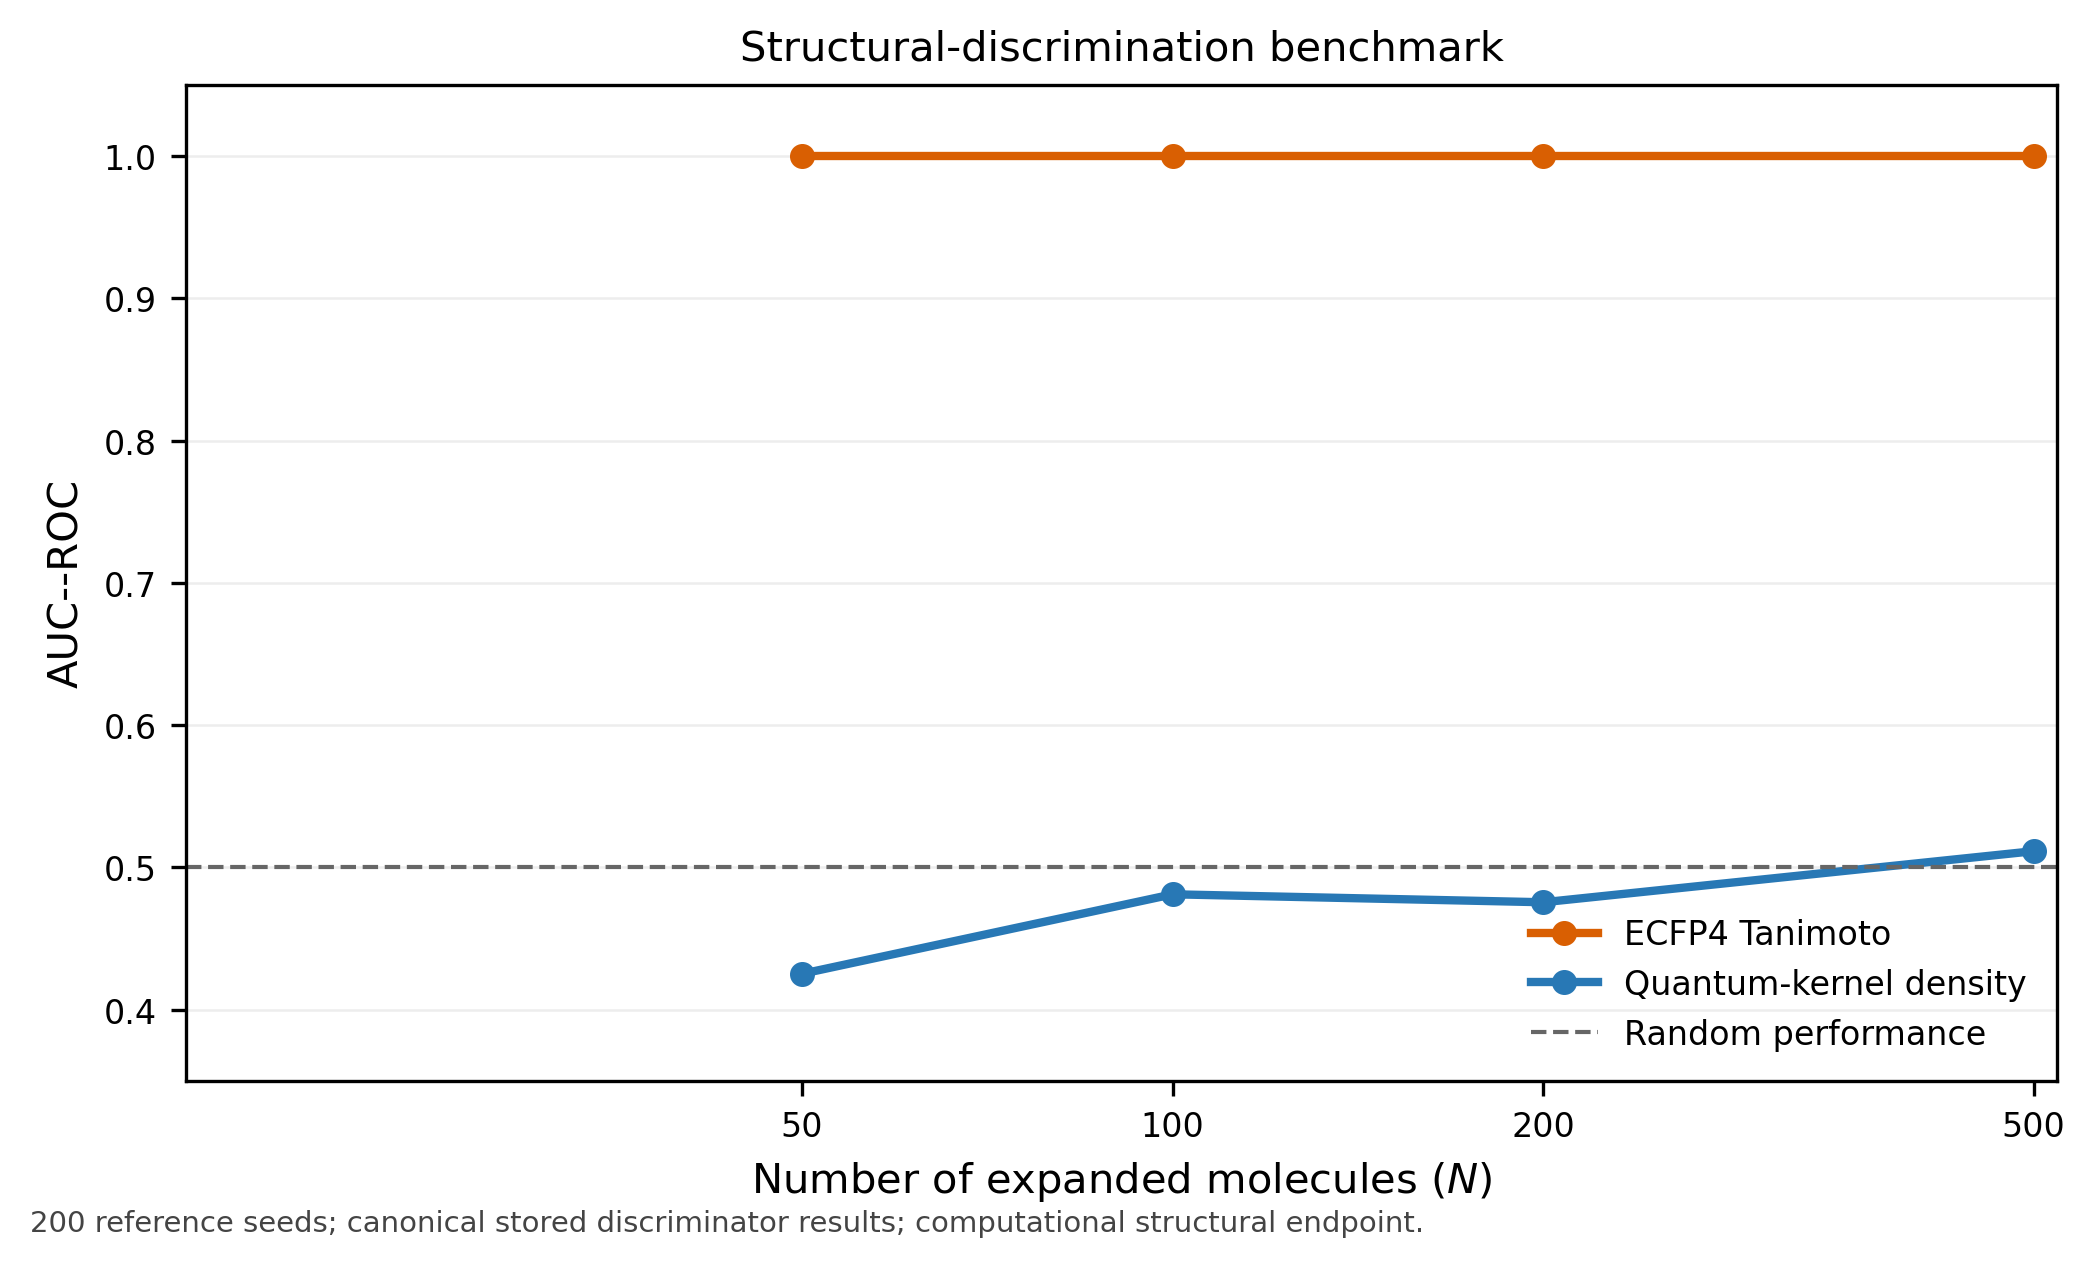
\includegraphics[width=0.80\textwidth]{p3_ga_discriminator.png}
\caption{Chemical-similarity versus quantum-kernel-density discriminator benchmark. ECFP4 Tanimoto distance (orange) and quantum-kernel density (blue) distinguish $N$ expanded molecules from \num{200} reference seeds; the dashed line marks random performance (AUC $= 0.5$). ECFP4 reached AUC $= 1.0$ at all tested $N$, whereas the quantum-kernel discriminator remained near random (AUC $= \numrange{0.425}{0.511}$). This is an honest negative: the quantum kernel in 8-d UMAP space lacks the atomic-level resolution to detect near-identical structural matches that ECFP4 captures trivially. The result is consistent with the canonical QKS finding (quantum $\approx$ RBF, $p > 0.05$) and confirms that quantum kernels do not improve structural discrimination for this generative protocol.}
\label{SM-fig:ga_discriminator}
\end{figure}


\section{Quantum circuit parameter optimisation}
\label{sec:qp_optimisation}

We compared \num{60} combinations of IQPEmbedding bond dimension ($d \in \{4,6,8\}$), repetition count ($n_{\text{rep}} \in \{1,2,3,4,6\}$), and kernel-PCA dimensionality ($n_{\text{kpca}} \in \{5,10,20,30\}$). Each combination was assessed by 5-fold stratified cross-validation with Random Forest on a \num{200}-molecule development subset; the selected configuration was subsequently evaluated on the \num{5000}-molecule panel.

The three highest-performing configurations are shown in \cref{tab:qp_optimisation}. The selected configuration ($d=6$, $n_{\text{rep}}=1$, $n_{\text{kpca}}=30$) achieved AUC $\num{0.8283}\pm\num{0.0371}$ on the \num{5000}-molecule panel. This result characterises the tested configuration and does not establish global optimality outside the present panel and protocol.

The full optimisation heatmap and marginal parameter-effect boxplots are provided in \cref{fig:qp_heatmap,fig:qp_effects}.

\begin{table}[htbp]
\centering
\caption{Quantum-kernel hybrid configurations. The three highest-performing configurations are shown for the \num{5000}-molecule evaluation panel (5-fold stratified cross-validation). The highest-performing configuration ($d=6$, $n_{\text{rep}}=1$, $n_{\text{kpca}}=30$) achieved AUC $\num{0.8283}\pm\num{0.0371}$. The development and evaluation panels differ from the primary benchmark in the main manuscript.}
\label{tab:qp_optimisation}
\begin{tabularx}{\textwidth}{S[table-format=1.0] S[table-format=1.0] S[table-format=2.0] S[table-format=1.4] S[table-format=1.4]}
\toprule
{$d$} & {$n_{\text{rep}}$} & {$n_{\text{kpca}}$} & {AUC} & {Std} \\
\midrule
6 & 1 & 30 & 0.8283 & 0.0371 \\
6 & 6 & 20 & 0.8047 & 0.0354 \\
6 & 6 & 30 & 0.8121 & 0.0396 \\
\bottomrule
\end{tabularx}
\vspace{1mm}
\footnotesize Values are from the \num{5000}-molecule evaluation panel (\num{3732} active and \num{1268} inactive). The panel and development subset differ in class proportions and selection criteria from the primary activity analysis; the values therefore describe configuration performance rather than final model performance.
\end{table}

\begin{figure}[htbp]
\centering
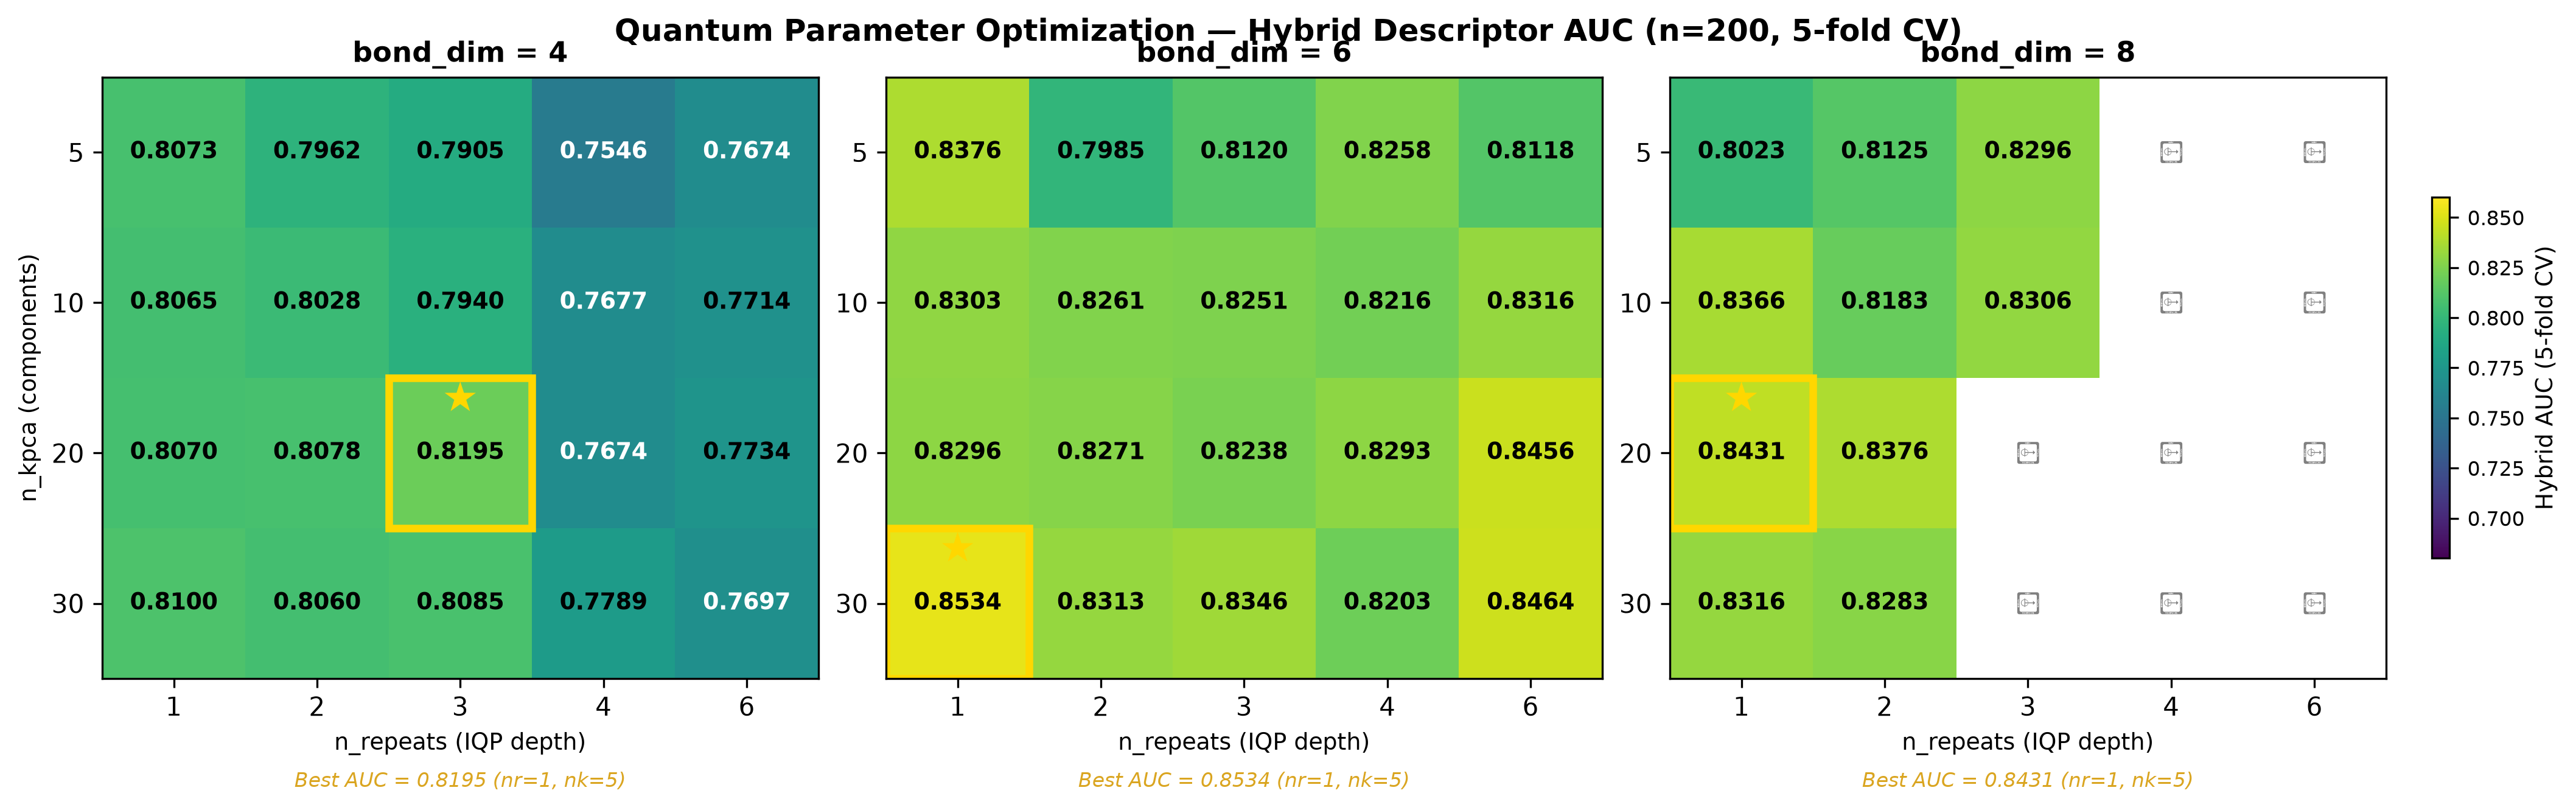
\includegraphics[width=0.80\textwidth]{p3_qp_optimization_heatmap.png}
\caption{Hybrid AUC heatmap across quantum circuit hyperparameters. Rows: bond dimension ($d$); columns: IQPEmbedding repeats ($n_{\text{rep}}$); colour: mean 5-fold AUC for each $n_{\text{kpca}}$ value. The gold cell marks the optimal configuration ($d = 6$, $n_{\text{rep}} = 1$, $n_{\text{kpca}} = 30$).}
\label{fig:qp_heatmap}
\end{figure}

\begin{figure}[htbp]
\centering
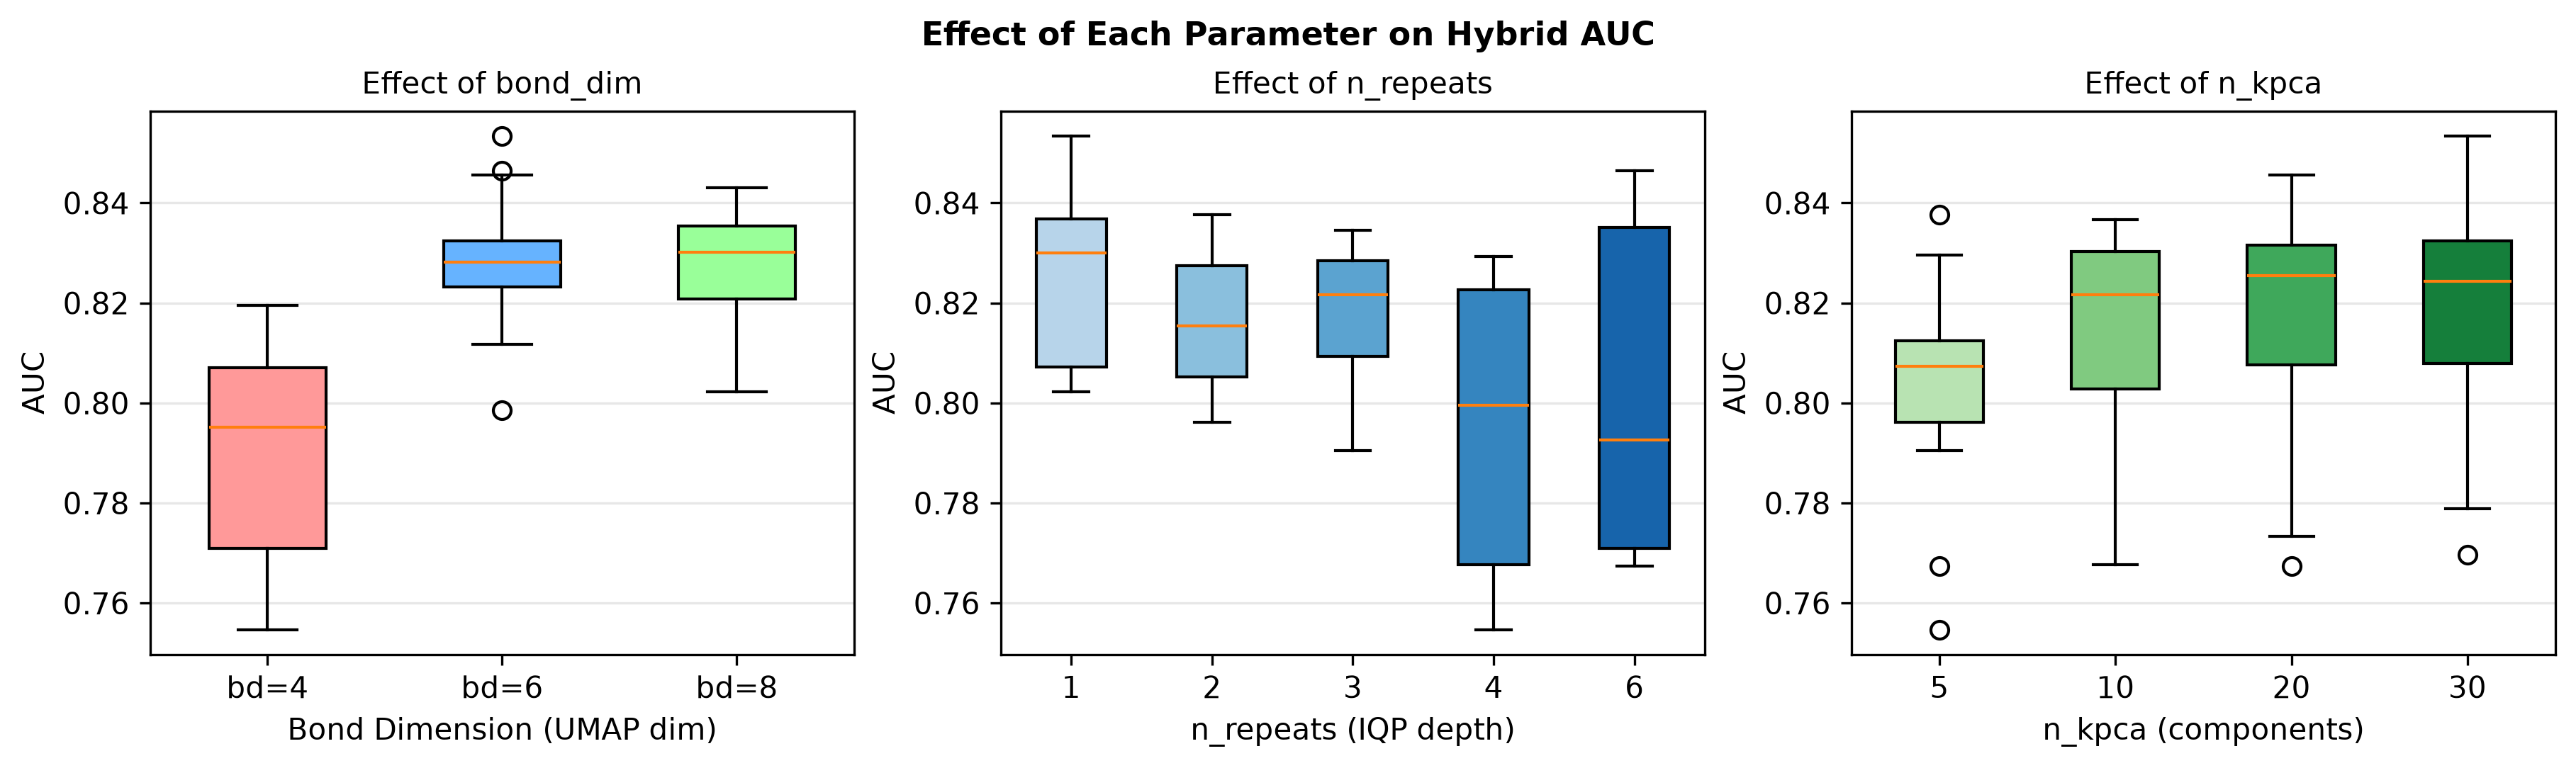
\includegraphics[width=0.80\textwidth]{p3_qp_parameter_effects.png}
\caption{Marginal AUC distributions per quantum circuit parameter. Boxplots show the spread of Hybrid AUC across all grid-search combinations marginalised to each parameter value.}
\label{fig:qp_effects}
\end{figure}


\section{Monte Carlo uncertainty estimation}
\label{sec:mc_uncertainty}

As a calibration analysis, we evaluated a Random Forest trained on the TFP+TNE representation using bootstrap resampling of \num{100} test molecules. The analysis used \num{50} bootstrap samples (fraction \num{0.7}, \num{30} trees per sample) and conformal prediction at $\alpha=0.05$. The resulting predictive uncertainty and coverage estimates are summarised in \cref{tab:mc_uncertainty}.

\begin{table}[htbp]
\centering
\caption{Bootstrap Monte Carlo uncertainty estimation results for the TFP+TNE descriptor (topological and tensor-network components of the hybrid) on the activity prediction task.}
\label{tab:mc_uncertainty}
\begin{tabularx}{\textwidth}{l S[table-format=1.4]}
\toprule
Metric & {Value} \\
\midrule
Bootstrap MC AUC & 0.5443 \\
Expected Calibration Error (ECE) & 0.0037 \\
\qty{95}{\percent} conformal coverage & \qty{95.0}{\percent} \\
Mean conformal set size & 1.820 \\
\bottomrule
\end{tabularx}
\vspace{1mm}
\footnotesize The low ECE and nominal conformal coverage indicate calibration in this secondary analysis, whereas the mean set size and weak uncertainty--error association (Spearman $\rho=-\num{0.286}$, $p=\num{0.004}$) indicate that uncertainty estimates did not reliably isolate misclassifications. This analysis complements, but does not replace, the held-out activity benchmark.
\end{table}


\section{Computational scalability}
\label{sec:scalability}

The measured computational costs of the three representation pipelines are summarised in \cref{tab:scalability}. Feature construction was approximately linear in library size, whereas formation of the dense quantum-kernel matrix followed $O(N^2)$ scaling.

\begin{table}[htbp]
\centering
\caption{Computational scalability of the representation pipelines. TDA and TNE timings were measured on the \num{19849}-molecule library; the QK timing is the per-fold kernel-matrix construction time for a \num{19849}-molecule fold using 32 parallel workers and a state-vector simulator.}
\label{tab:scalability}
\begin{tabularx}{\textwidth}{l l l l}
\toprule
Pipeline & {Wall time} & {Throughput} & {Scaling} \\
\midrule
TDA (persistent homology) & \SI{384}{\second} & 51.7~mol/s & Linear \\
TNE (Tucker decomposition) & \SI{488}{\second} & 40.7~mol/s & Linear \\
QK kernel matrix (per fold, $n=19{,}849$) & \SI{817}{\second} & $n^2/2$ pairs & $O(N^2)$ \\
\bottomrule
\end{tabularx}
\vspace{1mm}
\footnotesize Timings were measured on the full feature-generation library using the stated parallel configurations. The quadratic kernel cost motivates restricting QKS to smaller lead-optimisation panels unless approximate or batched kernel methods are introduced.
\end{table}


\section{Effect sizes for pairwise AUC comparisons}
\label{sec:effect_sizes}

Cohen's $d$ effect sizes for pairwise AUC comparisons against ECFP4 are reported in \cref{tab:effect_sizes}. These estimates use the \num{19836}-molecule classical benchmark (Random Forest, 5-fold stratified cross-validation) and are intended to complement, not replace, the fold-level uncertainty estimates.

% Auto-generated by p3_effect_sizes.py
% Effect sizes for all pairwise AUC comparisons (5-fold CV)

\begin{table}[htbp]
\centering
\caption{Effect sizes for pairwise AUC comparisons against ECFP4 baseline (19,849 molecules, 5-fold stratified CV). Cohen's $d$ quantifies the magnitude of difference; $>0.8$ indicates large effect.}
\label{tab:effect_sizes}
\begin{tabularx}{\textwidth}{l S[table-format=1.3] S[table-format=+1.3] S[table-format=+1.2] l S[table-format=1.4] S[table-format=1.3]}
\toprule
Method & {AUC} & {$\Delta$AUC} & {Cohen's $d$} & {Effect} & {$p$-value} & {Power} \\
\midrule
FCFP4 & 0.932 & +0.028 & +1.70 & large & 0.0189$^{*}$ & 0.809 \\
AP & 0.924 & +0.036 & +1.85 & large & 0.0145$^{*}$ & 0.864 \\
MACCS & 0.914 & +0.046 & +2.36 & large & 0.0062$^{*}$ & 0.970 \\
BPF & 0.904 & +0.056 & +2.87 & large & 0.0030$^{*}$ & 0.996 \\
TFP & 0.630 & +0.330 & +2.49 & large & 0.0051$^{*}$ & 0.981 \\
TNE & 0.630 & +0.330 & +2.49 & large & 0.0051$^{*}$ & 0.981 \\
PHCO & 0.912 & +0.048 & +2.92 & large & 0.0028$^{*}$ & 0.997 \\
Hybrid & 0.894 & +0.066 & +0.77 & medium & 0.1617 & 0.263 \\
TFP+ECFP4 & 0.950 & +0.010 & +0.63 & medium & 0.2302 & 0.195 \\
\bottomrule
\end{tabularx}
\vspace{1mm}
\footnotesize $^{*}$ $p < 0.05$ (uncorrected). Bonferroni-corrected $\alpha = 0.05/9 = 0.0056$. Power computed for 80\% target at $\alpha = 0.05$.
\end{table}




\section{ChEMBL enrichment analysis}
\label{sec:chembl_enrichment}

\cref{tab:chembl_enrichment} reports the enrichment of the Vina docking protocol for ChEMBL-annotated antimalarial actives and inactives across three Plasmodium targets.

\begin{table}[htbp]
\centering
\caption{ChEMBL enrichment screen for the Vina docking protocol using experimentally annotated antimalarial compounds. Enrichment is a computational docking-screen metric and should not be interpreted as experimental binding confirmation.}
\label{tab:chembl_enrichment}
\begin{tabularx}{\textwidth}{l c c c c l}
\toprule
Target & PDB & {Actives} & {Inactives} & {Enrichment} & Interpretation \\
\midrule
PfDHFR & 7F3Y & 53 & 18 & 5.43$\times$ & High estimate \\
PfATP4 & 9N10 & 73 & 87 & Not estimable & No inactive hits \\
PfCRT & 6UKJ & 12 & 19 & 1.46$\times$ & Below 2$\times$ \\
\bottomrule
\end{tabularx}
\vspace{1mm}
\footnotesize The estimates are descriptive and have no uncertainty intervals. For PfATP4, the denominator is zero because no inactive compound was recovered; the enrichment ratio is therefore undefined rather than infinite. These docking-screen results do not establish experimental binding.
\end{table}




\section{ChEMBL analogue novelty screen}
\label{sec:chembl_validation}

The top-10 candidates (\cref{tab:chembl_validation_top10}) were queried against three \textit{Plasmodium falciparum} targets (PfDHFR, PfCRT, PfATP4) through the ChEMBL REST API (release 37). All targets used the same Tanimoto threshold ($\geq 0.20$); PfClpP was not included because no corresponding \textit{P.~falciparum} ClpP target was available in ChEMBL. Only PfCRT returned analogues above the threshold. Ten candidate-level analogue records were retrieved, with some records referring to the same ChEMBL compound, and all were annotated as inactive. The analysis is therefore a novelty screen: it documents the absence of close active analogues in the queried records but does not measure activity of the proposed candidates.

\begin{table}[htbp]
\centering
\caption{ChEMBL analogue novelty screen for the top-10 candidates. The table lists the closest retrieved analogue with an experimental IC$_{50}$ annotation for each candidate-level record (Tanimoto threshold $\geq 0.20$). Only PfCRT yielded qualifying records; all were annotated as inactive (IC$_{50}$ 12.5--55~$\si{\micro\molar}$), and similarities were low (0.229--0.379). The screen supports chemical novelty relative to the queried records but does not test candidate activity.}
\label{tab:chembl_validation_top10}
\small
\begin{tabularx}{\textwidth}{c l l l l l}
\toprule
Rank & Target & ChEMBL ID & Activity & {IC$_{50}$ ($\mu$M)} & Tanimoto \\
\midrule
1 & PfCRT & CHEMBL4754685 & Inactive & 15.6 & 0.266 \\
2 & PfCRT & CHEMBL4754685 & Inactive & 15.6 & 0.235 \\
3 & PfCRT & CHEMBL4754685 & Inactive & 15.6 & 0.266 \\
4 & PfCRT & CHEMBL4745810 & Inactive & 12.5 & 0.250 \\
5 & PfCRT & CHEMBL4754685 & Inactive & 15.6 & 0.379 \\
6 & PfCRT & CHEMBL4754685 & Inactive & 15.6 & 0.239 \\
7 & PfCRT & CHEMBL4784051 & Inactive & 55.0 & 0.296 \\
8 & PfCRT & CHEMBL4754685 & Inactive & 15.6 & 0.229 \\
9 & PfCRT & CHEMBL4754685 & Inactive & 15.6 & 0.290 \\
10 & PfCRT & CHEMBL4754685 & Inactive & 15.6 & 0.270 \\
\bottomrule
\end{tabularx}
\vspace{1mm}
\footnotesize All retrieved records were annotated as inactive in ChEMBL. The low similarities indicate that no retrieved record was a close structural congener. This negative screen supports novelty relative to the queried records but does not measure activity. The machine-readable records are included with the supplementary data.
\end{table}



\section{Topological representation comparison}
\label{SM-sec:sota_benchmark}

\cref{SM-tab:sota} compares five persistent-homology vectorisation strategies. Random Forest was evaluated on the full \num{19849}-molecule feature library, whereas SVM was evaluated on a stratified $n=\num{5000}$ subsample because of kernel-matrix scaling. The two classifier blocks are presented separately because their populations and label distributions differ.

\begin{table}[htbp]
\centering
\caption{Comparison of five persistent-homology vectorisations (5-fold stratified cross-validation, class-weighted classifiers). Random Forest rows use the full \num{19849}-molecule feature library; SVM rows use a stratified $n=\num{5000}$ subsample. The classifier blocks have different populations and label distributions and should not be compared directly with one another or with the primary benchmark in the main manuscript (\cref{M-tab:benchmark}).}
\label{SM-tab:sota}
\begin{tabularx}{\textwidth}{l l S[table-format=1.4] S[table-format=1.4] S[table-format=1.4] S[table-format=1.0]}
\toprule
{Strategy} & {Classifier} & {AUC} & {Accuracy} & {F1} & {Features} \\
\midrule
PersStats & RF & 0.8731 & 0.8332 & 0.8906 & 22 \\
TFP-12 & RF & 0.8668 & 0.8275 & 0.8858 & 12 \\
TFP-Enriched & RF & 0.8666 & 0.8308 & 0.8887 & 32 \\
PersImage & RF & 0.8596 & 0.8265 & 0.8856 & 25 \\
BettiCurve & RF & 0.8110 & 0.7837 & 0.8557 & 20 \\
PersStats & SVM & 0.8042 & 0.7398 & 0.7436 & 22 \\
PersImage & SVM & 0.7912 & 0.7270 & 0.7312 & 25 \\
TFP-Enriched & SVM & 0.7891 & 0.7208 & 0.7250 & 32 \\
TFP-12 & SVM & 0.7857 & 0.7198 & 0.7220 & 12 \\
BettiCurve & SVM & 0.7198 & 0.6646 & 0.6620 & 20 \\
\bottomrule
\end{tabularx}
\vspace{1mm}
\footnotesize All classifiers used \texttt{class\_weight=balanced}. RF used $n_{\text{estimators}}=500$; SVM used an RBF kernel with $C=10$ and $\gamma=\texttt{scale}$. PersStats contains 22 persistence statistics, TFP-12 contains 12 homology summaries, TFP-Enriched contains 32 combined features, PersImage contains 25 features, and BettiCurve contains 20 features. The label proportions differ from those in the primary eOS80ch analysis.
\end{table}

Within the RF block, PersStats had the highest AUC among the topological strategies ($\num{0.8731}$), followed by TFP-12 ($\num{0.8668}$), TFP-Enriched ($\num{0.8666}$), PersImage ($\num{0.8596}$), and BettiCurve ($\num{0.8110}$). The corresponding SVM block showed the same broad ordering, although all SVM estimates were obtained on a different subsample. These results indicate that persistence summaries are useful complementary representations; they do not replace the primary comparison in the main manuscript, where the complete 78-feature TFP achieved AUC $\num{0.876}$ and ECFP4 remained strongest.


\section{TopologyNet analog: neural network on persistent homology features}

To compare PersStats with a neural-network classifier (TopologyNet~\citep{topologynet_2018}, D-GRIL~\citep{dgril_2026}), we benchmarked an MLP on the same 22 PersStats features. The MLP used 3 hidden layers (128, 64, 32 neurons), ReLU activation, class-balanced sample weighting, and early stopping (5-fold stratified CV, $n = \num{5000}$ subsample).

\begin{table}[htbp]
\centering
\caption{MLP versus Random Forest on 22 PersStats features ($n=\num{5000}$, 5-fold stratified cross-validation). RF AUC $= \num{0.860}$; MLP AUC $= \num{0.799}$ ($\Delta\mathrm{AUC}=-\num{0.061}$).}
\label{tab:topologynet_analog}
\begin{tabularx}{\textwidth}{l S[table-format=1.4] S[table-format=1.4] S[table-format=1.0]}
\toprule
{Classifier} & {AUC} & {Std} & {Features} \\
\midrule
Random Forest & 0.860 & 0.014 & 22 \\
MLP (128+64+32) & 0.799 & 0.015 & 22 \\
\bottomrule
\end{tabularx}
\end{table}

The MLP underperforms RF by $\Delta$AUC = $-0.061$, consistent with the broader benchmark finding that tree-based methods better capture PH feature interactions on summary statistics. TopologyNet~\citep{topologynet_2018} and D-GRIL~\citep{dgril_2026} operate on richer inputs (full persistence diagrams or multi-parameter persistence) where neural architectures may extract additional signal; on summary statistics alone, RF is the more appropriate classifier.

\vspace{4mm}


\section{Applicability domain and comparison with existing tools}

\subsection{Applicability domain analysis}

We used quantum-kernel density as a complementary applicability-domain diagnostic alongside classical fingerprint similarity. The density score $\rho(x)$ describes proximity to the empirical seed space in the simulated feature space; it is presented as a descriptive diagnostic rather than a validated applicability-domain metric.

\subsection{Comparison with existing tools}

To assess information retention after TNE compression, we analysed Tartarus docking scores \citep{tartarus_2024}: \num{19913} primary leads docked with QuickVina against three targets (1SYH/PfDHFR, 6Y2F/PfATP4, 4LDE/PfCRT). Random Forest regressors were trained on TNE-only vectors (\num{192}-dim) to predict each target's docking score, with ECFP4 as baseline.

For PfDHFR (1SYH), TNE achieved an R\textsuperscript{2} of \num{0.473} (Spearman $\rho = \num{0.695}$), slightly outperforming ECFP4 (R\textsuperscript{2} = \num{0.461}, $\rho = \num{0.689}$). For the remaining targets, ECFP4 maintained an advantage: 6Y2F (TNE R\textsuperscript{2} = \num{0.464} vs.\ ECFP4 \num{0.578}) and 4LDE (TNE R\textsuperscript{2} = \num{0.334} vs.\ ECFP4 \num{0.517}). These results show that the \num{15.6}$\times$ padded (\num{6.1}$\times$ real-atom mean) TNE compression retains information sufficient to predict docking scores on the same molecular set used to derive the embeddings, competitive with classical \num{2048}-bit fingerprints for specific targets. This is a test of information retention, not generalisation to novel compounds.

We next examined whether the Quantum Kernel Score captured polypharmacological docking profiles. Compounds were labelled as polypharmacological if they bound $\geq 2$ targets at $\Delta G \leq -\SI{7.0}{\kcalmol}$ (\qty{12.0}{\percent} prevalence in the merged $N=\num{17011}$ set). QKS remained within the variability of the tuned RBF comparator for this endpoint, which is interpreted as exploratory.

Persistent-homology features showed weak-to-moderate associations with the number of docking-defined targets across $N=\num{17011}$ molecules (\cref{fig:sm_tda_promiscuity}). The strongest associations were inverse correlations for H$_0$ count ($\rho=-\num{0.248}$), H$_0$ entropy ($\rho=-\num{0.243}$), and H$_1$ entropy ($\rho=-\num{0.190}$). The endpoint is a docking-derived target count rather than an experimental polypharmacology measurement; these associations are consequently hypothesis-generating and should not be interpreted as mechanistic rules.

\begin{figure}[htbp]
\centering
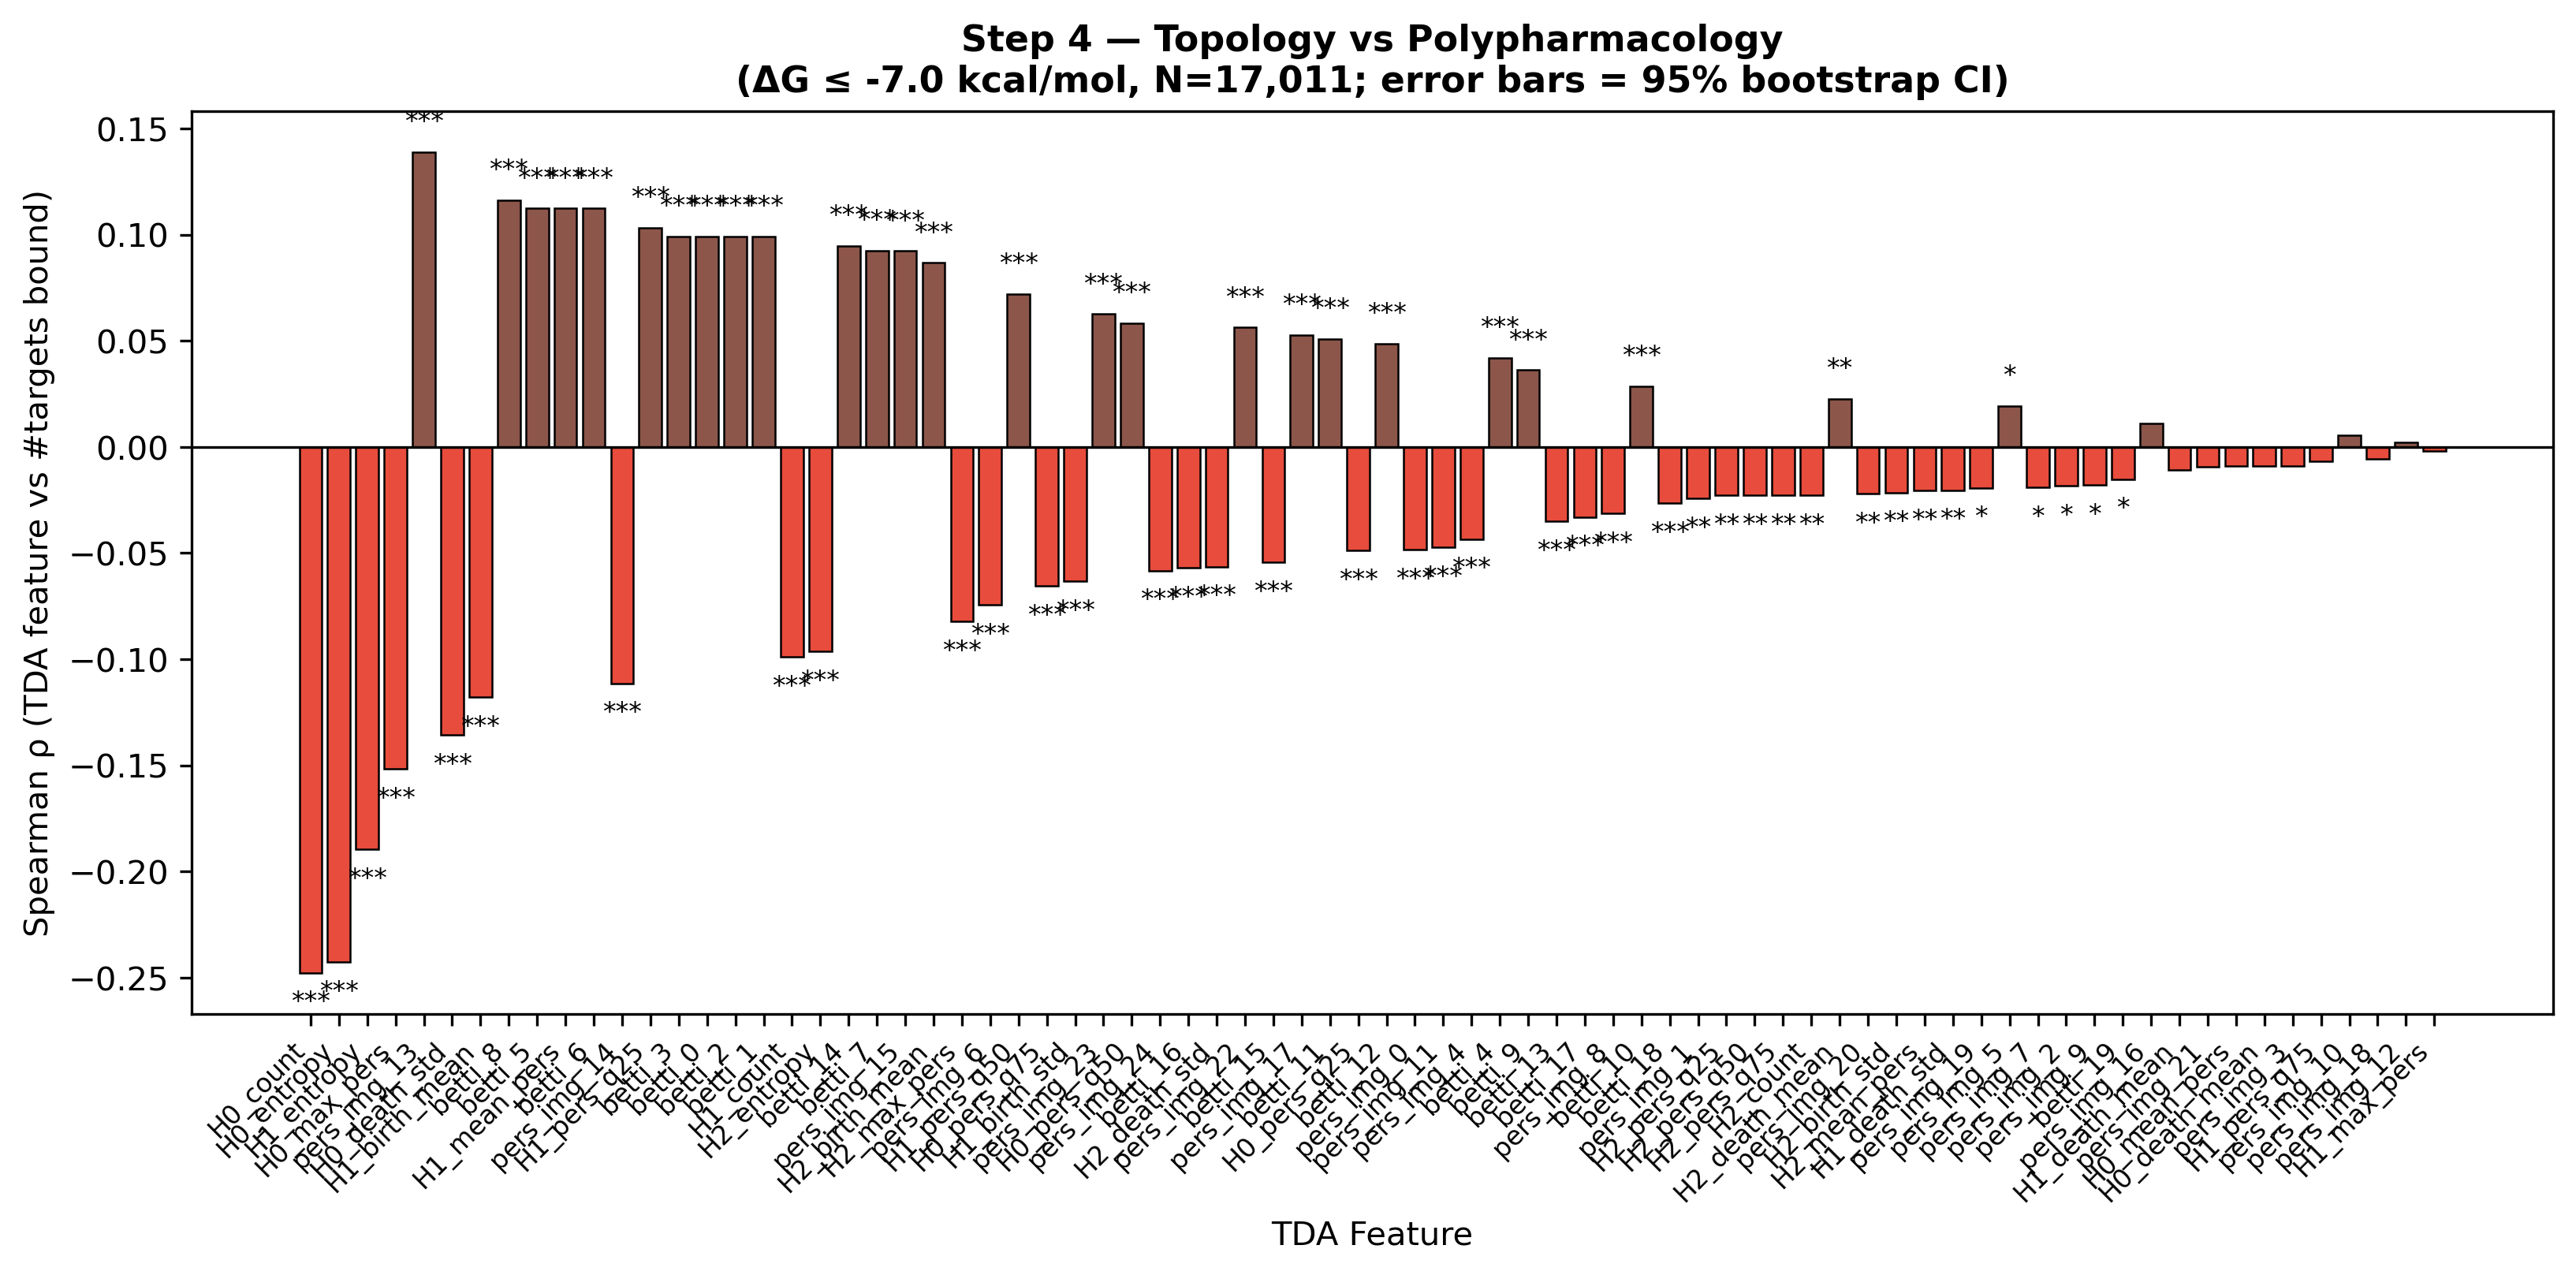
\includegraphics[width=0.80\textwidth]{p3_tda_promiscuity.png}
\caption{Exploratory associations between persistent-homology features and docking-defined target counts ($N=\num{17011}$). Bars show Spearman correlations with 95\% bootstrap intervals; the strongest inverse associations were H$_0$ count ($\rho=-\num{0.248}$), H$_0$ entropy ($\rho=-\num{0.243}$), and H$_1$ entropy ($\rho=-\num{0.190}$). The endpoint is computational docking, not experimental polypharmacology.}
\label{fig:sm_tda_promiscuity}
\end{figure}

\section{Extended analysis}

\subsection{Quantum kernel density vs classical fingerprint discriminator}

We compared quantum-kernel density with a classical chemical-similarity baseline \citep{jensen2019augmenting}. The comparison used $N = 50$, $100$, $200$, $500$ STONED-SELFIES-expanded molecules from \num{200} reference seeds. The classical baseline scored each molecule by its maximum ECFP4 Tanimoto similarity to any reference seed; the quantum kernel density scored each molecule by its mean kernel similarity to the reference set in the 8-qubit Hilbert space. Discriminator performance was measured as AUC-ROC.

The ECFP4 Tanimoto baseline achieved perfect separation (AUC $= \num{1.000}$) at all $N$ values, while the quantum kernel density achieved near-random performance (AUC $= \numrange{0.425}{0.511}$). The perfect Tanimoto score carries a caveat: with only two SELFIES-character mutations per molecule, a fraction of expanded molecules may be structurally identical to their seed. The quantum kernel density operates on an 8-dimensional UMAP-reduced feature space that discards the atomic-level resolution needed to detect near-identical structural matches. For applicability-domain assessment in generative protocols where expanded molecules are structurally close to training seeds, classical fingerprint-based distance metrics provide a simpler and more robust baseline.







\begin{figure}[htbp]
\centering
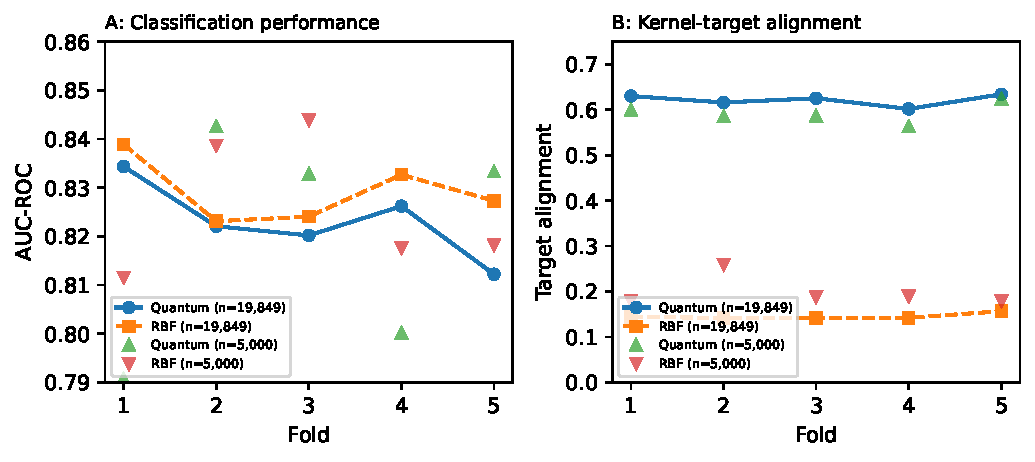
\includegraphics[width=0.75\textwidth]{applicability_domain.pdf}
\caption{(A) Classification performance per fold. AUC-ROC for quantum kernel and RBF kernel across 5-fold stratified cross-validation at $n = 19{,}849$ and $n = 5{,}000$. Quantum and RBF overlap at all folds (quantum $= 0.823 \pm 0.008$, RBF $= 0.829 \pm 0.007$; paired $t = -2.59$, $p = 0.060$, ns). (B) Kernel-target alignment per fold. The quantum kernel achieves substantially higher alignment ($0.622 \pm 0.013$) than RBF ($0.145 \pm 0.006$), yet this geometric advantage does not translate into classification performance ($\Delta$AUC $= -0.006$).}
\label{SM-fig:domain}
\end{figure}


\section{Quantum kernel circuit algorithm}
\label{sec:qkernel_algorithm}

\begin{algorithm}[htbp]
\caption{Quantum kernel circuit for 6-qubit state overlap using PennyLane's \texttt{IQPEmbedding} template.}
\label{SM-alg:qkernel}
\begin{algorithmic}[1]
\REQUIRE Data points $x_1, x_2 \in [-1, 1]^6$
\STATE Apply $\mathrm{IQPEmbedding}(weights, wires)$ parameterized by $x_1$
\STATE Apply $\mathrm{IQPEmbedding}^\dagger(weights, wires)$ parameterized by $x_2$
\STATE Measure probability of state $|000000\rangle$
\RETURN Kernel value $K(x_1, x_2)$
\end{algorithmic}
\end{algorithm}

The kernel value is $K(x_1, x_2) = |\langle \phi(x_1) | \phi(x_2) \rangle|^2$, estimated by the ground-state measurement probability, accelerated by PennyLane's \texttt{qp.kernels.kernel\_matrix}. Input vectors were computed as Morgan fingerprint atom-pair counts (radius 2, \num{2048} features) reduced to 6 dimensions by UMAP with Jaccard metric, then scaled to $[-1, 1]$.

\subsection{QKS benchmark protocol and state-vector kernel}
\label{sec:qks_benchmark}

\subsubsection{Evaluation protocol}
The kernel comparison (\cref{SM-tab:qkernel}) uses the same preprocessing and evaluation procedure as the hybrid analysis (\cref{sec:qp_optimisation}): 5-fold stratified cross-validation (\texttt{StratifiedKFold} with \texttt{random\_state=42}), UMAP reduction of the 2048-bit Morgan (radius 2) fingerprints to 6 dimensions (Jaccard metric, \texttt{random\_state=42}, $n_{\text{neighbors}}=15$, $min\_dist=0.1$) followed by scaling to $[-1,1]$, and support vector machines with precomputed kernels. The six-qubit circuit used one IQPEmbedding repeat. Benchmarks were run at two QKS panel sizes: the first \num{5000} molecules in library order (\num{3750} active, \num{1250} inactive) and the full representation panel of \num{19849} molecules. The complete-TNE intersection used for the canonical RF benchmark contains \num{19836} molecules (\num{14721} active, \num{5115} inactive).

The RBF baseline gamma was tuned by inner cross-validation on the grid $\{0.5, 1.0, 2.0, 5.0\}$. A linear kernel on the same $[-1,1]^6$ features served as an additional baseline. Paired fold comparisons gave quantum-versus-RBF $p=0.4186$ at $n=5000$ and $p=0.0604$ at $n=19849$; quantum-versus-linear comparisons gave $p=0.0002$ and $p=0.0006$, respectively. Target alignment was computed with the raw binary activity labels.

\subsubsection{State-vector kernel}
For computational tractability at $n=\num{5000}$ and $n=\num{19849}$, the pairwise IQPEmbedding circuit evaluation is replaced by a \textbf{state-vector kernel}: for each sample $x_i$, the 6-qubit state $|\phi(x_i)\rangle \in \mathbb{C}^{2^6}$ is obtained in a single circuit call, and the kernel matrix is formed as $K_{ij} = |V V^\dagger|^2$ where $V$ is the $N \times 64$ state matrix, via BLAS (approximately \num{1000}$\times$ faster than the pairwise evaluation). A small negative eigenvalue from floating-point noise is clipped by projecting onto the closest positive semi-definite matrix before the SVM is trained.

\subsubsection{Numerical consistency}
A numerical comparison of the state-vector and pairwise implementations on a 60-molecule, 5-fold dataset. The two implementations produced identical quantum-kernel AUCs ($\num{0.8756}\pm\num{0.0697}$) and target-alignment values under the raw binary-label convention. The \num{5000}-molecule and \num{19849}-molecule QKS analyses used the 6-qubit state-vector implementation for all five folds. The agreement supports numerical consistency; it does not estimate performance on an independent dataset.

\begin{table}[htbp]
\centering
\caption{Kernel comparison for activity prediction at two QKS panel sizes (5-fold cross-validation, 6-qubit IQPEmbedding, state-vector kernel; $n = \num{5000}$ and $n = \num{19849}$). The $n=\num{19849}$ QKS panel is the full representation panel; the primary RF analysis requiring complete TNE embeddings uses the $n=\num{19836}$ intersection reported in the main manuscript. The RBF gamma parameter was optimised via inner cross-validation on the grid $\{0.5, 1.0, 2.0, 5.0\}$ (per-fold best gamma at $n = \num{5000}$: 5, 1, 5, 5, 5). With the specified circuit, the gamma-tuned RBF kernel and the quantum kernel show \textbf{no statistically significant difference} at either scale ($p = \num{0.419}$ at $n = \num{5000}$; $p = \num{0.060}$ at $n = \num{19849}$, paired $t$-test; the latter a borderline trend toward lower QK performance), while the quantum kernel \textbf{significantly outperforms} the linear kernel at scale ($p \leq \num{0.0006}$). \textit{Interpretation:} with the specified circuit, the tuned RBF and quantum kernels were not detectably different at either scale, whereas the quantum kernel exceeded the linear comparator. These results are limited to the classically simulated 6-qubit protocol and do not establish quantum advantage.}
\label{SM-tab:qkernel}
\small
\begin{tabularx}{\textwidth}{l *{4}{>{\centering\arraybackslash}X} >{\raggedright\arraybackslash}X}
\toprule
Kernel & {\shortstack{AUC\\$n=5000$}} & {\shortstack{TA\\$n=5000$}} & {\shortstack{AUC\\$n=19849$}} & {\shortstack{TA\\$n=19849$}} & {$p$ vs. RBF} \\
\midrule
Quantum (IQPEmbedding, 6 qubits) & 0.820 & 0.592 & 0.823 & 0.622 & $p=0.419/0.060$, n.s. \\
RBF (gamma-tuned, SVM) & 0.826 & 0.199 & 0.829 & 0.145 & --- \\
Linear & 0.517 & --- & 0.537 & --- & $p<0.001$ \\
\bottomrule
\end{tabularx}
\vspace{1mm}
\footnotesize Paired $t$-test (5 folds), quantum versus linear: $p = \num{0.0002}$ ($n = \num{5000}$) and $p = \num{0.0006}$ ($n = \num{19849}$), both significant. Quantum target alignment (\numrange{0.592}{0.622}) exceeds RBF target alignment (\numrange{0.145}{0.199}) yet does not translate into a discrimination advantage.
\end{table}


\begin{figure}[htbp]
\centering
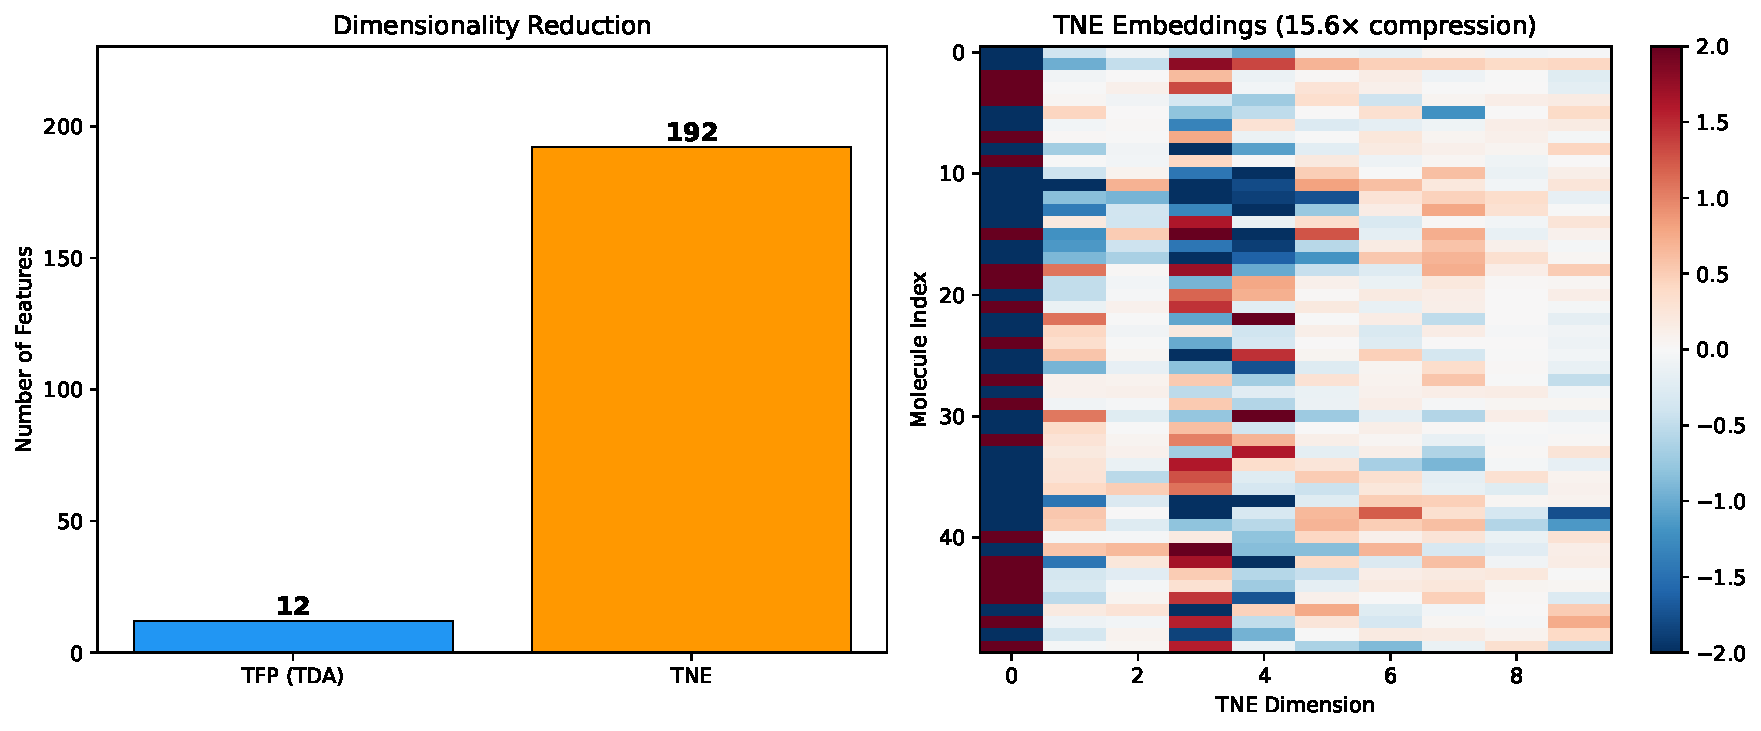
\includegraphics[width=0.75\textwidth]{tensor_compression.pdf}
\caption{Compression ratio and reconstruction error versus Tucker bond dimension. At $d=8$, the physically meaningful mean real-atom compression ratio is \num{6.1}$\times$ (based on $\sim$\num{39} mean atoms per molecule), with a reconstruction error of \num{0.113}. (See main manuscript Methods Section~2.4.2 for discussion of the mathematical padding convention).}
\label{SM-fig:tensor}
\end{figure}

\begin{figure}[htbp]
\centering
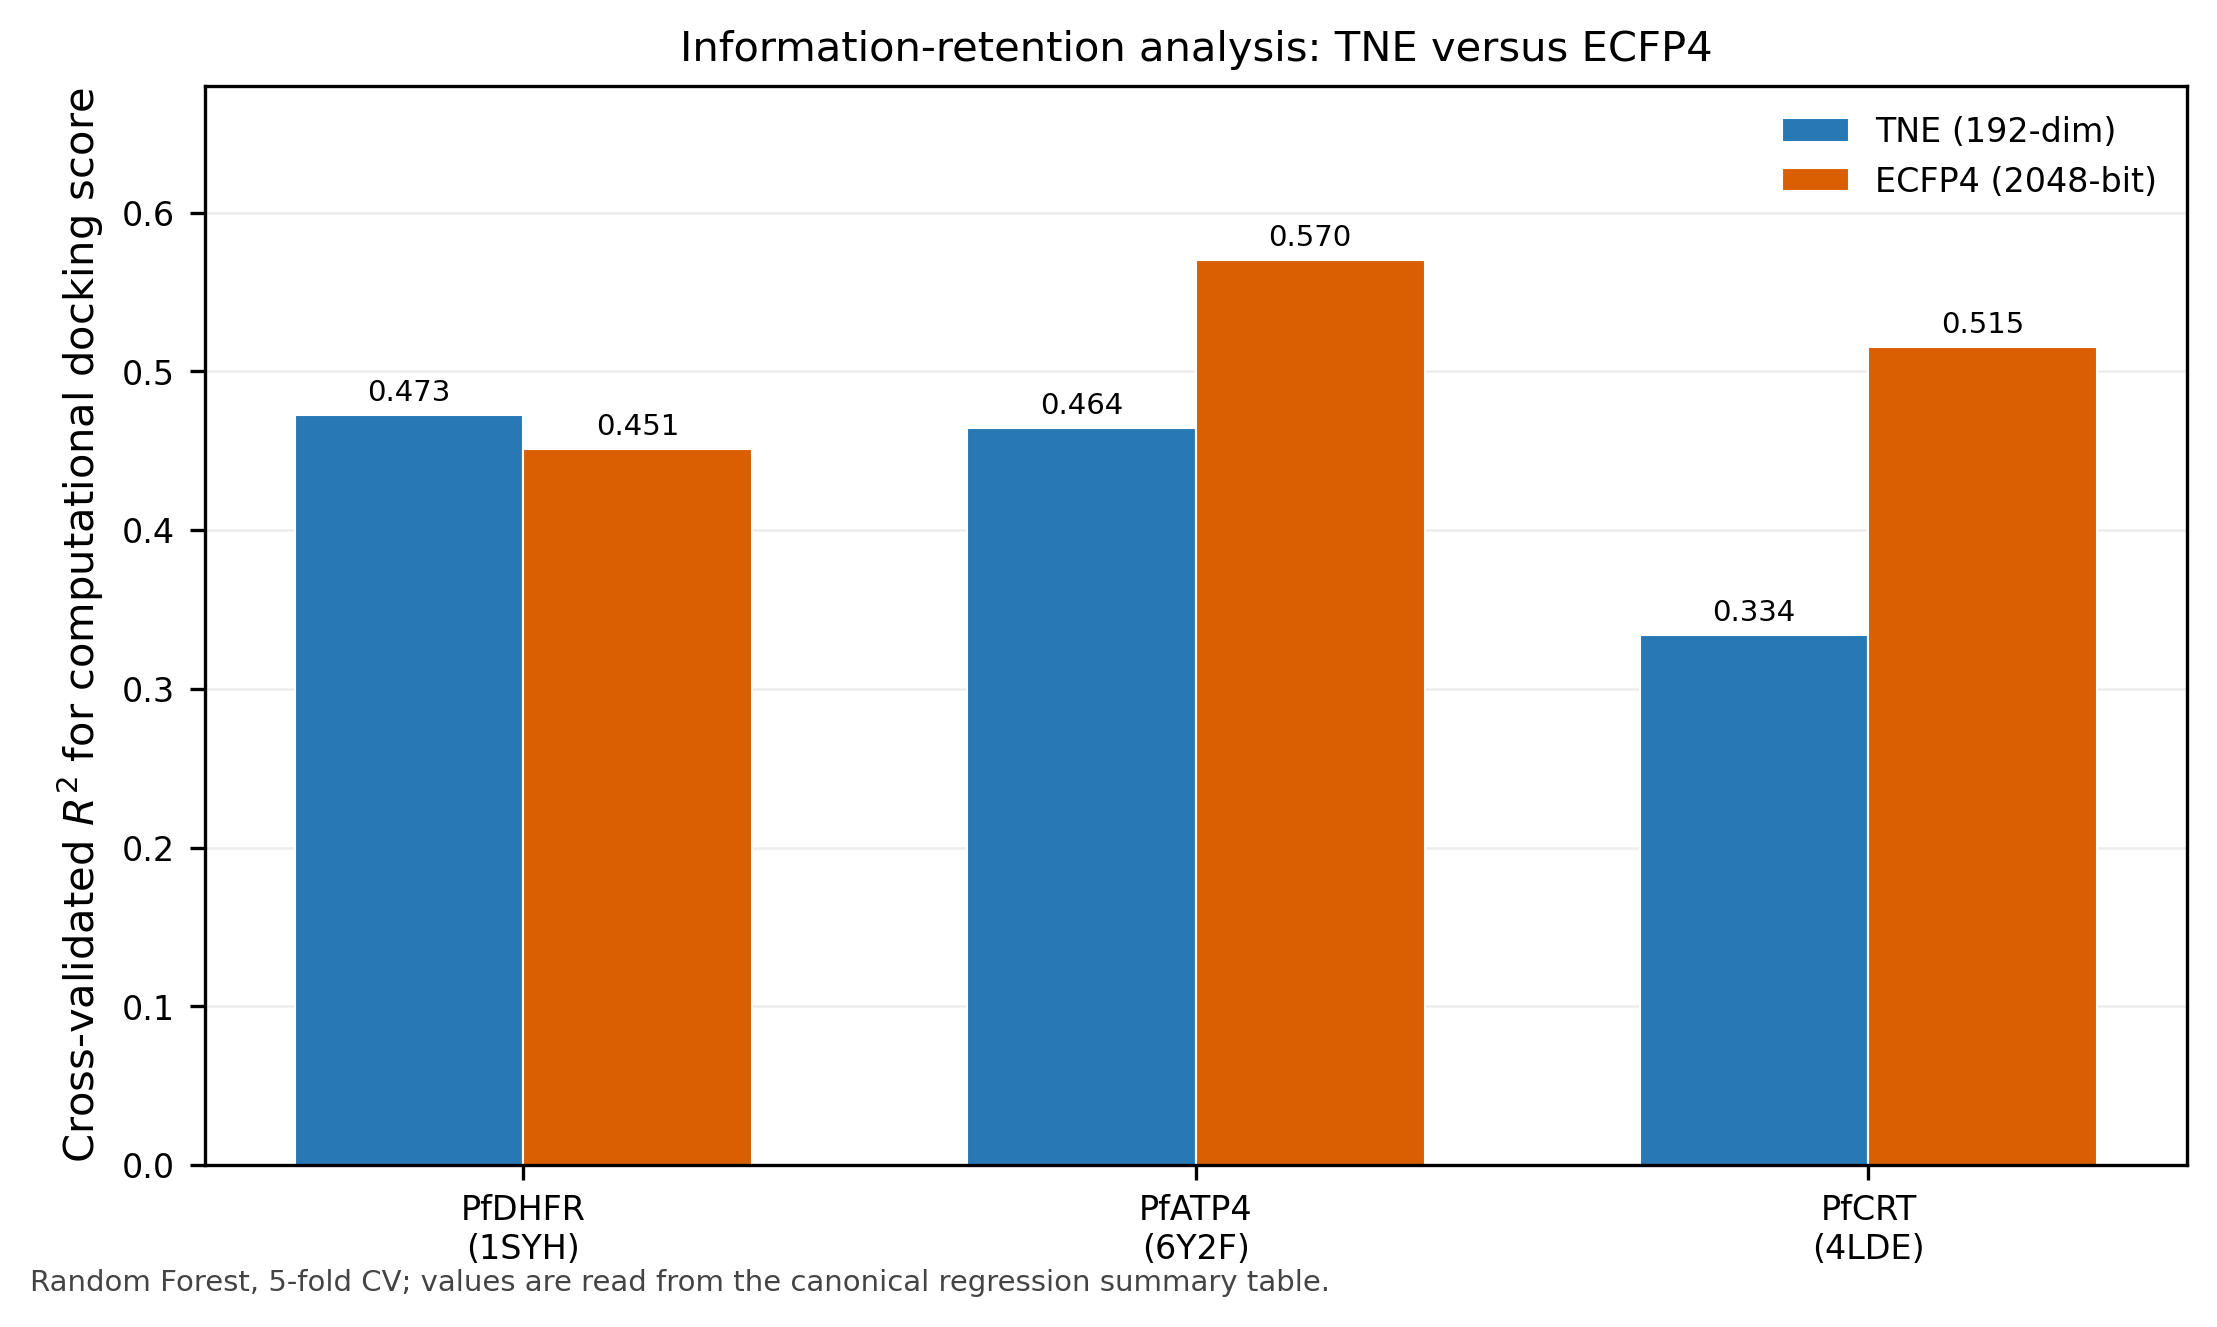
\includegraphics[width=0.80\textwidth]{p3_tne_regression_summary.png}
\caption{Information-retention analysis for 192-dimensional Tensor Network Embeddings. Bars show cross-validated $R^2$ values for TNE and ECFP4 regressors predicting computational QuickVina docking scores for three \textit{Plasmodium} targets. TNE was competitive for PfDHFR but lower than ECFP4 for PfATP4 and PfCRT; the analysis is descriptive and does not establish experimental binding or prospective generalisation.}
\label{SM-fig:tne_parity}
\end{figure}


\section{Transfer analysis under a ChEMBL label-source shift}

\subsection{Descriptor transfer analysis}

All descriptor methods were evaluated on an external ChEMBL antimalarial dataset ($n = \num{22447}$) using 5-fold stratified cross-validation with Random Forest (\num{200} trees, \texttt{random\_state=42}). The external panel was assembled from ChEMBL~34 bioactivity records for \textit{Plasmodium falciparum} assays (IC$_{50} \leq \SI{10}{\micro\molar}$ = active, $> \SI{10}{\micro\molar}$ = inactive). It is external to the primary eOS80CH label source; molecule-level disjointness was not established and is not claimed. Feature extraction followed the identical pipeline used for the internal benchmark. For the intention-to-evaluate analysis, TNE embedding failures ($n = \num{351}$, \qty{1.6}{\percent}) were assigned zero vectors. The complete-case analysis ($n = \num{22096}$) gave ECFP4 \num{0.960}, TFP \num{0.861}, TNE \num{0.644}, and TFP+TNE \num{0.798}, versus ITT values of \num{0.960}, \num{0.864}, \num{0.645}, and \num{0.800}. The qualitative ranking was unchanged.

\begin{table}[htbp]
\centering
\caption{Descriptor transfer under the ChEMBL label-source shift. Random Forest estimates are shown for the intention-to-evaluate panel ($n=\num{22447}$) and the complete-case sensitivity panel ($n=\num{22096}$). Internal values are included for context; molecule-level disjointness was not established. TNE failures were retained as zero-vector penalties in the primary analysis.}
\label{SM-tab:extval_descriptor}
\small
\begin{tabularx}{\textwidth}{l *{3}{>{\centering\arraybackslash}X}}
\toprule
Method & {\shortstack{Internal AUC\\$n=19836$}} & {\shortstack{Transfer AUC\\$n=22447$}} & {$\Delta$} \\
\midrule
ECFP4   & 0.948 & 0.960 & +0.012 \\
TFP     & 0.876 & 0.865 & -0.011 \\
TNE     & 0.722 & 0.645 & -0.077 \\
TFP+TNE & 0.888 & 0.800 & -0.088 \\
\bottomrule
\end{tabularx}
\end{table}

\subsection{Quantum-kernel transfer analysis}

The quantum kernel was evaluated on the ChEMBL label-source-shift panel (ITT $n = \num{22447}$, 5-fold SVM with precomputed kernels) following the specified protocol from \cref{sec:qks_benchmark}: UMAP reduction of 2048-bit Morgan fingerprints to 6 dimensions (Jaccard metric, \texttt{random\_state=42}, $n_{\text{neighbors}}=15$, $min\_dist=0.1$), scaling to $[-1,1]$, and the 6-qubit IQPEmbedding state-vector kernel. The RBF gamma was tuned by inner cross-validation on the grid $\{0.5, 1.0, 2.0, 5.0\}$.

\begin{table}[htbp]
\centering
\caption{Kernel transfer under the ChEMBL label-source shift (5-fold SVM, $n=\num{22447}$). QKS was lower than RBF (AUC $\num{0.817}$ versus $\num{0.847}$); the corrected-resampled comparison was exploratory ($p=\num{0.021}$). Internal values are shown for context, and classifier differences prevent direct comparison with the descriptor-transfer table.}
\label{SM-tab:extval_qks}
\small
\begin{tabularx}{\textwidth}{l *{3}{>{\centering\arraybackslash}X}}
\toprule
Kernel & {Internal AUC} & {Transfer AUC} & {$p$ vs. RBF} \\
\midrule
Quantum (6 qubits) & 0.823 & 0.817 & {$p_{\mathrm{corr}}=\num{0.021}$} \\
RBF & 0.829 & 0.847 & {---} \\
Linear & 0.537 & 0.544 & {$p<\num{0.001}$} \\
\bottomrule
\end{tabularx}
\vspace{1mm}
\footnotesize Internal: $n=\num{19849}$; transfer: $n=\num{22447}$. The corrected-resampled comparison is exploratory; classifier and population differences limit cross-table comparisons.
\end{table}

\subsection{H$_1$--RRS association is size-mediated}
\label{sec:tda_rrs}

The Spearman correlation between H$_1$ count and resistance-resilience scores (RRS) \citep{temgoua2027md} was examined in two cohorts: (i)~an expanded cohort of $n = \num{494}$ compounds with complete H$_1$ and continuous RRS profiles (used for the cross-paper analysis in \cref{fig:h1_rrs}), and (ii)~a subset of $N = \num{77}$ compounds with validated per-target RRS classification (used for the H$_1$--RRS association in \cref{sec:tda_rrs}). In the expanded cohort ($n = \num{494}$), H$_1$ count showed a weak unadjusted association with continuous RRS (Spearman $\rho = \num{0.2399}$, $p = \num{6.76e-8}$), but the partial association was null after controlling for molecular weight, ring count, fraction sp$^3$, and H$_0$ count ($\rho_{\text{partial}} = \num{0.0329}$, $p = \num{0.4668}$). In the validated subset ($N = \num{77}$), the raw correlation was $\rho = \num{0.312}$ ($p = \num{0.006}$) but dropped to $\rho_{\text{partial}} = \num{0.033}$ ($p = \num{0.47}$) after the same adjustment. Both analyses converge on the same conclusion: the H$_1$--RRS association is mediated by molecular complexity rather than topological structure per se. This result does not support a direct H$_1$--RRS association but is consistent with the broader finding that topological complexity correlates with binding promiscuity (\cref{M-sec:tda_promiscuity}).

\bibliographystyle{unsrtnat}
\bibliography{Bibliography_Paper3}

\end{document}
